
\documentclass[11pt,a4paper]{article}
\usepackage{C}



\begin{document}
\clearpage\clearpage\setcounter{page}{1}\pagestyle{HTML}
\section{Introducci\'on al Lenguaje C}
El lenguaje de programaci\'on C fue creado por Dennis Ritchie en 1972 en
Bell Telephone Laboratories, con el objetivo de reescribir un sistema
operativo, el UNIX, en un lenguaje de alto nivel, para poder adaptarlo
(\textit{portarlo}) a diferentes arquitecturas. Por este motivo sus
creadores se propusieron metas de dise\~no especiales, tales como: 

\liststyleLii
\begin{itemize}
\item {\bfseries
Posibilidad de acceder al {\textquotedbl}bajo nivel{\textquotedbl}
(poder utilizar todos los recursos del hardware). }
\item {\bfseries
C\'odigo generado eficiente en memoria y tiempo (programas peque\~nos y
veloces) }
\item {\bfseries
Compilador portable (implementable en todas las arquitecturas) }
\end{itemize}

La primera definici\'on oficial del lenguaje fue dada en 1978 por
\textbf{Brian Kernighan y Dennis Ritchie} en su libro {\textquotedbl}El
lenguaje de programaci\'on C{\textquotedbl}. Este lenguaje fue llamado
{\textquotedbl}C K\&R{\textquotedbl}. En 1983 se cre\'o el comit\'e
ANSI que en 1988 estableci\'o el standard ANSI C, con algunas reformas
sobre el C K\&R. Simult\'aneamente Kernighan y Ritchie publicaron la
segunda edici\'on de su libro, describiendo la mayor parte de las
caracter\'isticas del ANSI C. 

\begin{flushleft}
\tablehead{~
 &
\begin{center}
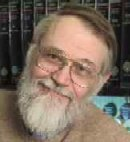
\includegraphics[width=3.44cm,height=3.757cm]{img/kernighan.jpg}
\end{center}
 &
~
 &
\begin{center}
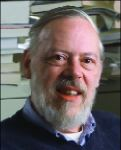
\includegraphics[width=3.201cm,height=3.969cm]{img/dennis_ritchie.jpg}
\end{center}
 &
~
\\}
\begin{supertabular}{m{2.192cm}m{5.395cm}m{2.192cm}m{5.03cm}m{2.192cm}}
~
 &
\centering \itshape Brian Kernighan &
~
 &
\centering \itshape Dennis Ritchie &
~
\\
\end{supertabular}
\end{flushleft}
Actualmente existen implementaciones de C para todas las arquitecturas y
sistemas operativos, y es el lenguaje m\'as utilizado para la
programaci\'on de sistemas. Por su gran eficiencia resulta ideal para
la programaci\'on de sistemas operativos, drivers de dispositivos,
herramientas de programaci\'on. El 95\% del sistema operativo UNIX
est\'a escrito en C, as\'i como la gran mayor\'ia de los modernos
sistemas y ambientes operativos y programas de aplicaci\'on que corren
sobre ellos.\newline
\href{info/info1.html#info1}{Mas informaci\'on ...} 

\subsection[Caracter\'isticas del lenguaje]{Caracter\'isticas del
lenguaje}
C es un lenguaje compilado. A nivel sint\'actico, presenta grandes
similitudes formales con Pascal, pero las diferencias entre ambos son
importantes. A pesar de permitir operaciones de bajo nivel, tiene las
estructuras de control, y permite la estructuraci\'on de datos, propias
de los lenguajes procedurales de alto nivel como Pascal. 

Un programa en C es, por lo general, m\'as sint\'etico que en otros
lenguajes procedurales como Pascal; la idea central que atraviesa todo
el lenguaje es la minimalidad. La definici\'on del lenguaje consta de
muy pocos elementos; tiene muy pocas palabras reservadas. Como rasgo
distintivo, en C no existen, rigurosamente hablando, funciones o
procedimientos de uso general del programador. Por ejemplo, no tiene
funciones de entrada/salida; la definici\'on del lenguaje apenas
alcanza a las estructuras de control y los operadores. La idea de
definir un lenguaje sin funciones es, por un lado, hacer posible que el
compilador sea peque\~no, f\'acil de escribir e inmediatamente
portable; y por otro, permitir que sea el usuario quien defina sus
propias funciones cuando el problema de programaci\'on a resolver tenga
requerimientos especiales. 

Sin embargo, se ha establecido un conjunto m\'inimo de funciones,
llamado la \textbf{biblioteca standard} del lenguaje C, que todos los
compiladores proveen, a veces con agregados. La filosof\'ia de la
biblioteca standard es la portabilidad, es decir, casi no incluye
funciones que sean espec\'ificas de un sistema operativo determinado.
Las que incluye est\'an orientadas a la programaci\'on de sistemas, y a
veces no resultan suficientes para el programador de aplicaciones. No
provee, por ejemplo, la capacidad de manejo de archivos indexados, ni
funciones de entrada/salida interactiva por consola que sean seguras
({\textquotedbl}a prueba de usuarios{\textquotedbl}). Esta deficiencia
se remedia utilizando bibliotecas de funciones {\textquotedbl}de
terceras partes{\textquotedbl} (creadas por el usuario u obtenidas de
otros programadores). 

El usuario puede escribir sus propios procedimientos (llamados
\textbf{funciones} aunque no devuelvan valores). Aunque existe la
noci\'on de bloque de sentencias, el lenguaje se dice \textit{no}
estructurado en bloques porque no pueden definirse funciones dentro de
otras. Las funciones de la biblioteca standard no tienen ning\'un
privilegio sobre las del usuario y sus nombres no son palabras
reservadas; el usuario puede reemplazarlas por sus propias funciones
simplemente d\'andoles el mismo nombre. 

El lenguaje entrega completamente el control de la m\'aquina subyacente
al programador, no realizando controles de tiempo de ejecuci\'on. Es
decir, no verifica condiciones de error comunes como \textit{overflow}
de variables, errores de entrada/salida, o consistencia de argumentos
en llamadas a funciones. Como resultado, es frecuente que el
principiante, y aun el experto, cometan errores de programaci\'on que
no se hacen evidentes enseguida, ocasionando problemas y costos de
desarrollo. Permite una gran libertad sint\'actica al programador. No
es fuertemente tipado. Cuando es necesario, se realizan conversiones
autom\'aticas de tipo en las asignaciones, a veces con efectos
laterales inconvenientes si no se tiene precauci\'on. Una funci\'on que
recibe determinados par\'ametros formales puede ser invocada con
argumentos reales de otro tipo. 

Se ha dicho que estas caracter\'isticas
{\textquotedbl}liberales{\textquotedbl} posibilitan la realizaci\'on de
proyectos complejos con m\'as facilidad que otros lenguajes como Pascal
o Ada, m\'as estrictos; aunque al mismo tiempo, as\'i resulta m\'as
dif\'icil detectar errores de programaci\'on en tiempo de
compilaci\'on. En este sentido, seg\'un los partidarios de la
tipificaci\'on estricta, C no es un buen lenguaje. Gran parte del
esfuerzo de desarrollo del standard ANSI se dedic\'o a dotar al C de
elementos para mejorar esta deficiencia. 

Los tipos de datos no tienen un tama\~no determinado por la definici\'on
del lenguaje, sino que diferentes implementaciones pueden adoptar
diferentes convenciones. Parad\'ojicamente, esta caracter\'istica
obedece al objetivo de lograr la portabilidad de los programas en C. El
programador est\'a obligado a no hacer ninguna suposici\'on sobre los
tama\~nos de los objetos de datos, ya que lo contrario har\'ia al
software dependiente de una arquitectura determinada. 

Una caracter\'istica especial del lenguaje C es que el pasaje de
argumentos a funciones se realiza siempre por valor. ?`Qu\'e ocurre
cuando una funci\'on debe modificar datos que le son pasados como
argumentos? La \'unica salida es pasarle -por valor- la direcci\'on del
dato a modificar. Las consecuencias de este hecho son m\'as fuertes de
lo que parece a primera vista, ya que surge la necesidad de todo un
conjunto de t\'ecnicas de manejo de punteros que no siempre son bien
comprendidas por los programadores poco experimentados, y abre la
puerta a sutiles y escurridizos errores de programaci\'on. Quiz\'as
este punto, junto con el de la ausencia de chequeos en tiempo de
ejecuci\'on, sean los que le dan al C fama de {\textquotedbl}dif\'icil
de aprender{\textquotedbl}. 

Por \'ultimo, el C no es un lenguaje orientado a objetos, sino que
adhiere al paradigma tradicional de programaci\'on procedural. No
soporta la orientaci\'on a objetos propiamente dicha, al no
proporcionar herramientas fundamentales, como la herencia. Sin embargo,
algunas caracter\'isticas del lenguaje permiten que un proyecto de
programaci\'on se beneficie de todas maneras con la aplicaci\'on de
algunos principios de la orientaci\'on a objetos, tales como el
ocultamiento de informaci\'on y el encapsulamiento de
responsabilidades. El lenguaje C++, orientado a objetos, \textbf{no }es
una versi\'on m\'as avanzada del lenguaje o un compilador de C con
m\'as capacidades, sino que se trata de un lenguaje completamente
diferente. 

Algunas nuevas caracter\'isticas de C99 son: 

\liststyleLiii
\begin{itemize}
\item Matrices de tama\~no variable 
\item Soporte de n\'umeros complejos 
\item Tipos \textbf{long long int} y \textbf{unsigned long long int} de
al menos 64 bits 
\item Familia de funciones \textbf{vscanf()} 
\item Comentarios al estilo de C++ prefijando las l\'ineas con la
secuencia {\textquotedbl}//{\textquotedbl}. 
\item Familia de funciones \textbf{snprintf()} 
\item Tipo boolean
\end{itemize}
~ 

\subsection[El ciclo de compilaci\'on]{El ciclo de compilaci\'on}
Las herramientas esenciales de un ambiente de desarrollo, adem\'as de
cualquier editor de textos, son el \textbf{compilador}, el
\textbf{linkeditor} o \textit{linker} y el \textbf{bibliotecario}. A
estas herramientas b\'asicas se agregan otras, \'utiles para
automatizar la compilaci\'on de proyectos extensos, almacenar y
recuperar versiones de programas fuente, chequear sintaxis en forma
previa a la compilaci\'on, etc. Seg\'un el ambiente operativo y
producto de software de que se trate, estas herramientas pueden
encontrarse integradas en una interfaz de usuario uniforme, en modo
texto o gr\'afico, o ser comandos de l\'inea independientes, con
salidas de texto simples. 

\subsubsection{Compilador}
El compilador acepta un archivo fuente, posiblemente relacionado con
otros (una \textbf{unidad de traducci\'on}), y genera con \'el un
\textbf{m\'odulo objeto}. Este m\'odulo objeto contiene porciones de
c\'odigo ejecutable mezclado con referencias, a\'un no resueltas, a
variables o funciones cuya definici\'on no figura en los fuentes de
entrada. Estas referencias quedan en forma simb\'olica en el m\'odulo
objeto hasta que se resuelvan en un paso posterior. 

\subsubsection[Linkeditor o linker]{Linkeditor o \textit{linker}}
El linkeditor recibe como entrada un conjunto de m\'odulos objeto y
busca resolver, o enlazar, las referencias simb\'olicas en ellos,
buscando la definici\'on de las variables o funciones faltantes en los
mismos objetos o en bibliotecas. Estas pueden ser la biblioteca
standard u otras provistas por el usuario. Cuando encuentra la
definici\'on de un objeto buscado (es decir, de una variable o
funci\'on), el linker la copia en el archivo resultante de salida (la
\textit{resuelve}). El objetivo del linker es resolver todas las
referencias pendientes para producir un programa ejecutable. 

\subsubsection{Bibliotecario}
El bibliotecario es un administrador de m\'odulos objeto. Su funci\'on
es reunir m\'odulos objeto en archivos llamados bibliotecas, y luego
permitir la extracci\'on, borrado, reemplazo y agregado de m\'odulos.
El conjunto de m\'odulos en una biblioteca se completa con una tabla de
informaci\'on sobre sus contenidos para que el linker pueda encontrar
r\'apidamente aquellos m\'odulos donde se ha definido una variable o
funci\'on, y as\'i extraerlos durante el proceso de linkedici\'on. El
bibliotecario es utilizado por el usuario cuando desea mantener sus
propias bibliotecas. La creaci\'on de bibliotecas propias del usuario
ahorra tiempo de compilaci\'on y permite la distribuci\'on de software
sin revelar la forma en que se han escrito los fuentes y
protegi\'endolo de modificaciones. 

\begin{flushleft}
\tablehead{~
\\}
\begin{supertabular}{m{17.8cm}}
\raggedleft\arraybslash 
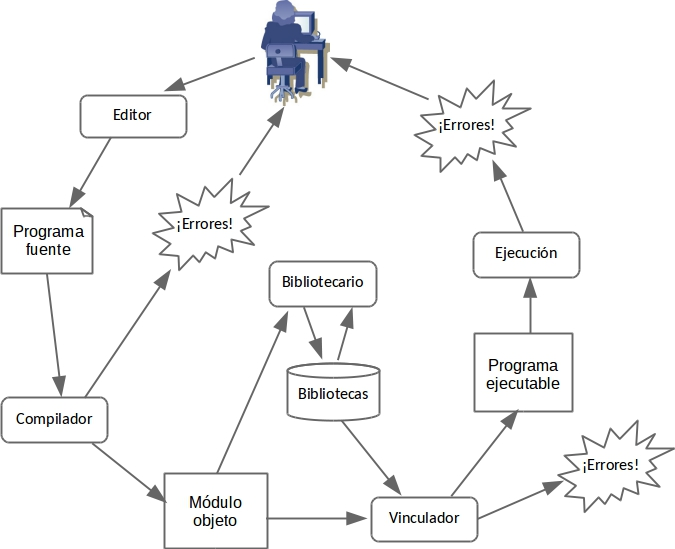
\includegraphics[width=12.303cm,height=9.155cm]{img/ciclo.jpg} \\
\centering\arraybslash El ciclo de compilaci\'on produce un ejecutable a
partir de archivos fuente\\
\end{supertabular}
\end{flushleft}
~ 

\subsection[El primer ejemplo]{El primer ejemplo}
El cl\'asico ejemplo de todas las introducciones al lenguaje C es el
programa \textbf{hello.c}:

{\ttfamily\bfseries\color{black}
\#include {\textless}stdio.h{\textgreater}}

{\ttfamily\bfseries\color{black}
/* El primer programa! */}

{\ttfamily\bfseries\color{black}
main()}

{\ttfamily\bfseries\color{black}
\{}

{\ttfamily\color{black}
\ \ \ \ \ \ \ \ \textbf{printf({\textquotedbl}Hola,
gente!{\textbackslash}n{\textquotedbl});}}

{\ttfamily\bfseries\color{black}
\}}

%\newline
Ejecute los siguientes pasos para ver el primer ejemplo en C funcionando


\liststyleLiv
\begin{itemize}
\item 1.Bajar el archivo \href{ejemplos/hola.c}{hola.c} ~ y guardar
en~el directorio local de trabajo
\item 2.~ Sin cambiarde directorio, ejecutar el comando:

\textstyleEmphasis{\textbf{\textcolor{black}{\$ make hola}}}
\item 3. Finalmente ejecutar el programa asi:

% \textstyleEmphasis{\textbf{\textcolor{black}{\$ ./hola}}}\textcolor{black}{ ~}~~~~ (el . significa el directorio actual
de trabajo)
\end{itemize}
%\newline
Se puede hacer lo mismo de esta manera: 

\liststyleLv
\begin{itemize}
\item 1.~ Bajar el archivo~ \href{ejemplos/hola.c}{hola.c} ~ y guardar
en~el directorio local de trabajo
\item 2.~ Sin cambiar de directorio, ejecutar el comando:

\textstyleEmphasis{\textbf{\textcolor{black}{\$ gcc hola.c~ - o~ hola}}}
\item 3. Finalmente ejecutar el programa asi:

% \textstyleEmphasis{\textbf{\textcolor{black}{\$./hola}}}\textcolor{black}{~~}~~~~~
(el . significa el directorio actual de trabajo) 
\end{itemize}
\newline
La diferencia es que en el primer caso utilizamos la herramienta
\href{info/info1.html#info3}{\textstyleEmphasis{make (mas
informaci\'on)}} que nos asiste en la compilaci\'on de proyectos,
mientras que en el segundo caso invocamos directamente al compilador.
En este \'ultimo caso, le decimos al compilador (gcc)~que compile el
archivo hola.c y que la salida (-o de out) se llame hola. Probar que
ocurre si hacemos: gcc hola.c.\newline
En el~primer caso el utilitario
\href{info/info1.html#info4}{\textstyleEmphasis{make}} hace todo esto
por nosotros.~~ 

\newline
\textstyleStrongEmphasis{Funcionamiento el programa} 

\liststyleLvii
\begin{itemize}
\item Este programa minimal comienza con una \textbf{directiva de
preprocesador} que indica incluir en la unidad de traducci\'on al
archivo \textit{header} \textbf{stdio.h}. Este contiene, entre otras
cosas, la declaraci\'on (o \textbf{prototipo}) de la funci\'on de
salida de caracteres \textbf{printf}. Los prototipos se incluyen para
advertir al compilador de los tipos de las funciones y de sus
argumentos. 
\item Entre los pares de caracteres especiales \textbf{/*} y \textbf{*/
}se puede insertar cualquier cantidad de l\'ineas de comentarios. 
\item La funci\'on \textbf{main()} es el cuerpo principal del programa
(es por donde comenzar\'a la ejecuci\'on). Terminada la ejecuci\'on de
main(), terminar\'a el programa. 
\item La funci\'on printf() imprimir\'a la cadena entre comillas, que es
una \textbf{constante string} terminada por un car\'acter de
\textbf{nueva l\'inea} (la secuencia especial
{\textquotedbl}{\textbackslash}n{\textquotedbl}). 
\end{itemize}
\newline
~ 

% \subsection[Mapa de memoria de un programa Mas informaci\'on ... ]{Mapa de memoria de un programa \href{info/info1.html#info2}{Mas informaci\'on ...} }

\bigskip


\bigskip

~ 

\subsection[Ejercicios]{Ejercicios}
1. ?`Qu\'e nombres son adecuados para los archivos fuente C? 

2. Describa las etapas del ciclo de compilaci\'on. 

3. ?`Cu\'al ser\'ia el resultado de: 

\liststyleLviii
\begin{itemize}
\item Editar un archivo fuente? 
\item Ejecutar un archivo fuente? 
\item Editar un archivo objeto? 
\item Compilar un archivo objeto? 
\item Editar una biblioteca?
\end{itemize}
4. ?`Qu\'e pasar\'ia si un programa C \textbf{no} contuviera una
funci\'on \textbf{main()}?.~~Haga la prueba con~
\href{ejemplos/hola.c}{hola.c} ~ 

5. Edite el programa \textbf{hola.c} y modif\'iquelo seg\'un las pautas
que siguen. Interprete los errores de compilaci\'on. Si resulta un
programa~ejecutable, vea qu\'e hace el programa. 

\liststyleLix
\begin{itemize}
\item Quite los par\'entesis de main() 
\item Quite la llave izquierda de main() 
\item Quite las comillas izquierdas 
\item Quite los caracteres
{\textquotedbl}{\textbackslash}n{\textquotedbl} 
\item Agregue al final de la cadena los caracteres
{\textquotedbl}{\textbackslash}n{\textbackslash}n{\textbackslash}n{\textbackslash}n{\textquotedbl}

\item Agregue al final de la cadena los caracteres
{\textquotedbl}{\textbackslash}nAdi\'os
mundo!{\textbackslash}n{\textquotedbl} 
\item Quite las comillas derechas 
\item Quite el signo punto y coma. 
\item Quite la llave derecha de main() 
\item Agregue un punto y coma en cualquier lugar del texto 
\item Agregue una coma o un d\'igito en cualquier lugar del texto 
\item Reemplace la palabra \textbf{main} por \textbf{program},
manteniendo los par\'entesis. 
\item Elimine la apertura o cierre de los comentarios
\end{itemize}
\href{adicionales/adic1.html#adic1}{Ejercicios
Adicionales}\href{adicionales/adic1.html#adic1}{\textcolor{black}{
}}\href{adicionales/adic1.html#adic1}{\newline
}\newline
\href{adicionales/adic1.html#adic2}{Ejercicios Avanzados}


\bigskip


\bigskip
\end{document}
